\documentclass[a4paper,10pt,twocolumn]{article}
\usepackage[T1]{fontenc}
\usepackage[utf8]{inputenc}
\usepackage[italian]{babel}
\usepackage[top=3cm, bottom=3cm, left=2.5cm, right=2.5cm]{geometry}
\usepackage{graphicx}
\graphicspath{ ./images/} 
\usepackage{subfig}
\usepackage{dblfloatfix}
\usepackage[hidelinks]{hyperref}

\begin{document}

\title{SIR Simulation}
\author{Lorenzo Manini \and Nicolò Montalti}
\date{A.A. 2019/2020}

\maketitle

\section{Descrizione del progetto}
Il progetto consiste in una libreria dedicata allo sviluppo di simulazioni basate sul modello SIR. 

\subsection*{Organizzazione del codice}
Il codice è stato sviluppato collaborando su GitHub. La repository è pubblica e liberamente consultabile al link in \cite{bib:GitHub}.

Il sorgente è suddiviso in tre cartelle: include, src e tests. Le dichiarazione delle classi sono contenute negli header all'interno di include/, mentre la loro implementazione è nei cpp contenuti in src/. Tutti i file utili al testing sono invece raggruppati in tests/. Infine, una copia di questa relazione è contenuta nella cartella tex/.

\subsection*{Struttura del programma}
\subsubsection*{La popolazione}
La simulazione ha come “attori” istanze di \emph{Person}. Una \emph{Person} contiene una posizione, una velocità ed alcune informazioni relative allo stato di infezione. In particolare la variabile membro \emph{Sub Status} è un enumeratore che definisce una sotto categoria di S, I o R. Ad esempio, gli infetti sono divisi in \emph{incubation}, per le quali il virus è nella fase di incubazione, \emph{infective}, cioè in grado di infettare altre persone, e \emph{quarantined}, cioè in quarantena. Ogni \emph{Person} è contenuta in un std::vector<Person>, che ha come alias \emph{People}. Infine, lo struct \emph{Population}, che rappresenta l’intera popolazione, contiene tre oggetti \emph{People} denominati rispettivamente S, I e R. I \emph{Person} contenuti in S sono considerati sani, quelli contenuti in I infetti e quelli in R recuperati.

\subsubsection*{La simulazione}
La classe che permette all’utente di creare e far avanzare la simulazione è \emph{Simulation}. La classe ha tre variabili membro private, che vengono inizializzate dal costruttore:
\begin{itemize}
    \item Simulation\_State state: contiene tutte le informazioni riguardanti lo stato della simulazione
    \item G\_ Motion\& motion: referenza al modulo che implementa il movimento della popolazione
    \item G\_ Infection\& infection: referenza al modulo che implementa l’evoluzione dell’infezione
\end{itemize}

\emph{Simulation State} è uno struct che contiene un’istanza di \emph{Population}, la dimensione dello spazio della simulazione e il tempo a cui fa riferimento quello stato. Lo spazio in cui avviene la simulazione è stato modellizzato come un piano cartesiano di estremi 0 e \emph{size} su entrambi gli assi; una persona in un \emph{Simulation State} deve sempre trovarsi all’interno di questo spazio. Il tempo è invece stato discretizzato in ticks interi; i ticks di un \emph{Simulation State} non possono diminuire.

\emph{G Motion} e \emph{G Infection} sono classi astratte nelle quali è dichiarata una funzione membro pubblica virtuale \emph{update}. Una implementazione di \emph{G Motion}, quando viene chiamato \emph{update(Population}\& \emph{population, int size)}, deve aggiornare la posizione dei \emph{Person} contenuti nella referenza a \emph{Population}. La nostra libreria fornisce \emph{Random Motion}. Una implementazione di \emph{G Infection}, quando viene chiamato \emph{update(Population}\& \emph{population, int ticks)}, deve far progredire l’infezione. Questo avviene spostando i \emph{Person} tra i vari \emph{People} (S, I, R) e aggiornando le variabili membro dedicate dei \emph{Person}. La libreria fornisce \emph{Simple Infection} e \emph{Incubation Infection}.

Prima di inizializzare un’istanza di \emph{Simulation}, l’utente deve creare due istanze di classi che implementano rispettivamente \emph{G Motion} e \emph{G Infection} e un \emph{Simulation State} iniziale. A questo punto è possibile creare un’istanza di \emph{Simulation} passando i tre oggetti come parametri al costruttore.

\emph{Simulation} ha a sua volta una funzione membro pubblica \emph{update()}, che chiama gli \emph{update} delle istanze di \emph{G Motion} e \emph{G Infection} e incrementa i ticks. In questo modo l’utente, dopo aver creato l’istanza di \emph{Simulation}, deve solo chiamare \emph{Simulation::update()} per far progredire la simulazione di un tick alla volta.
\emph{Simulation} ha inoltre una funzione membro pubblica \emph{is\_over()} che ritorna true se non ci sono più infetti nella popolazione.

\subsubsection*{Output grafico}
La libreria mette a disposizione due classi per visualizzare l’andamento della simulazione. La spiegazione dettagliata degli output, con alcuni esempi, è fornita nella sezione Risultati (\ref{sec:risultati}).

Le due classi che gestiscono la grafica sono \emph{Display} e \emph{Plot}. \emph{Display}, basata sulla libreria grafica SFML, permette di visualizzare in tempo reale i \emph{Person} come cerchi colorati che si muovono in un piano. \emph{Plot}, basata sul framework di ROOT, permette invece di visualizzare in tempo reale un grafico con l’andamento del numero di sani, infetti e recuperati. Tramite la funzione membro \emph{Plot::save()} è inoltre possibile salvare il grafico come RootFile e i dati dell’andamento come csv.

Entrambe le classi funzionano in modo analogo. È necessario passare al costruttore una referenza costante allo stato della simulazione che si vuole visualizzare. Questa è ottenibile tramite la funzione membro \emph{Simulation::get\_state()}. Dopodiché, per aggiornare ciò che viene mostrato, è sufficiente chiamare rispettivamente \emph{Display::update()} e \emph{Plot::update()}.


\section{Compilazione ed esecuzione}
La compilazione è gestita tramite CMake. Per compilare il codice è sufficiente creare una directory di build, generare il Makefile tramite CMake e compilare con make.

\begin{verbatim}
    mkdir build
    cd build
    cmake ..
    make
\end{verbatim}

Affinché la compilazione abbia successo, è necessario avere installato sul proprio computer CMake 3.16 o superiore \cite{bib:CMake}, SFML 2.5 o superiore \cite{bib:SFML} e ROOT \cite{bib:ROOT}. Il programma è stato testato su Ubuntu 18.04 LTS e Ubuntu 20.04 LTS. Si suggerisce di utilizzare quest'ultima versione, se possibile, per via della maggior compatibilità con SFML 2.5.

L'eseguibile del main viene generato nella cartella build/, mentre i test in build/tests. Per eseguire il programma è quindi sufficiente spostarsi nella directory di build e digitare

\begin{verbatim}
    ./SIR_simulation
\end{verbatim}

Si apriranno due finestre, una con la schematizzazione delle persone e una con i grafici. Chiudendo la finestre dei grafici si termina l'intera applicazione, mentre chiudendo quella con la popolazione si interrompe la sola simulazione, lasciando la possibilità di interagire con il grafico per eseguire un fit o per salvare i dati.

I test possono essere eseguiti singolarmente, a partire dagli eseguibili generati in build/tests/, o collettivamente con

\begin{verbatim}
    make test
\end{verbatim}

Eseguendo il codice con l'address sanitizer abilitato, si è notato che la terminazione della applicazione da parte di ROOT comporta dei memory leak. Si è concluso che essi siano dovuti a librerie esterne, in particolare a libfontconfig. Il problema sembra circoscritto alla classe \emph{Plot}.

\section{Risultati}
\label{sec:risultati}
L'applicazione restituisce due tipi di output grafici. Nella prima finestra vengono mostrate le persone, schematizzate come cerchi colorati, che si muovono in uno spazio quadrato. Lo stato delle persone è indicato con colori diversi: verde per i sani, rosso per gli infettivi, arancione se il virus è in incubazione, bianco per la quarantena e blu per i recuperati. Un'immagine d'esempio è mostrata in fig. \ref{fig:display}. Contemporaneamente, in una seconda finestra, viene mostrato un grafico aggiornato in tempo reale in cui viene plottato il numero di sani, infetti e recuperati.

\begin{figure}
    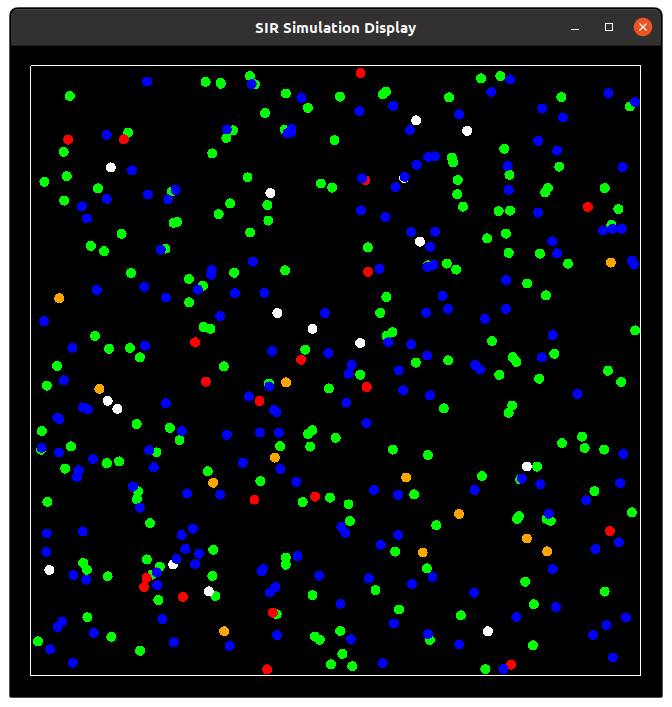
\includegraphics[width=\linewidth]{images/display.png}
    \caption{Finestra grafica ottenuta dalla classe Display. Il verde corrisponde ai sani, il rosso agli infettivi, l'arancione al virus in incubazione, il bianco alla quarantena e il blu ai guariti}
    \label{fig:display}
\end{figure}

Di seguito vengono riportati gli esiti di alcune simulazioni effettuate variando i parametri delle classi \emph{Infection} e \emph{Motion}. Se non diversamente indicato, i parametri  dello stato iniziale sono size = 600, S = 400, I = 10 e  R = 0. Si è scelto di iniziare la simulazione con 10 individui infettivi per velocizzarne l'esecuzione. Inoltre si è notato che  con un solo infetto può capitare che questo guarisca prima di infettare altre persone. Quest'ultimo caso, sebbene possibile, è stato ritenuto di scarso interesse.

La classe \emph{Random Motion} è stata inizializzata con una deviazione standard pari a 0.2. Si è notato che variare questo parametro influisce poco sulla simulazione. L'unica differenza apprezzabile è nella durata dell'epidemia, che diminuisce all'aumentare della varianza.

La classe \emph{Simple Infection} è stata inizializzata con una distanza critica di 10, una probabilità di infezione di 0.05 e un tempo di recupero di media 200 e deviazione standard 50. Inoltre, alla variante \emph{Incubation Infection}, si sono assegnati un tempo di incubazione di 50 e una probabilità di essere costretti alla quarantena di 0.005.

L'esito di una simulazione con i parametri sopra descritti e la classe \emph{Simple Infection} a gestire l'infezione è riportato in fig. \ref{fig:simple_005}. In fig. \ref{fig:simple_008} si può vedere come aumentando la probabilità di infezione a 0.08 il picco si alzi sensibilmente.

Diminuire la size da 600 a 400, come mostrato in fig- \ref{fig:simple_400}, determina un'epidemia molto più violenta, con un picco alto e la totalità della popolazione che contrae il virus. Aumentarla a 800 (fig. \ref{fig:simple_800}), simulando una sorta di distanziamento sociale, provoca invece l'effetto opposto.

Introducendo un periodo di incubazione si ottiene il grafico in fig. \ref{fig:incubation}, in cui si può notare come l'intensità dell'epidemia sia più modesta. Infine, aggiungendo la possibilità di essere costretti alla quarantena, si ottiene il grafico in fig. \ref{fig:quarantine}, in cui il numero di infetti è costantemente sotto controllo e il numero finale di individui che non contraggono il virus consistente. Inoltre, il tempo di durata dell'epidemia è più del doppio di quello della versione senza quarantena.

\begin{figure*}[p]
    \centering
    \subfloat[][Probabilità: 0.05\label{fig:simple_005}]{
        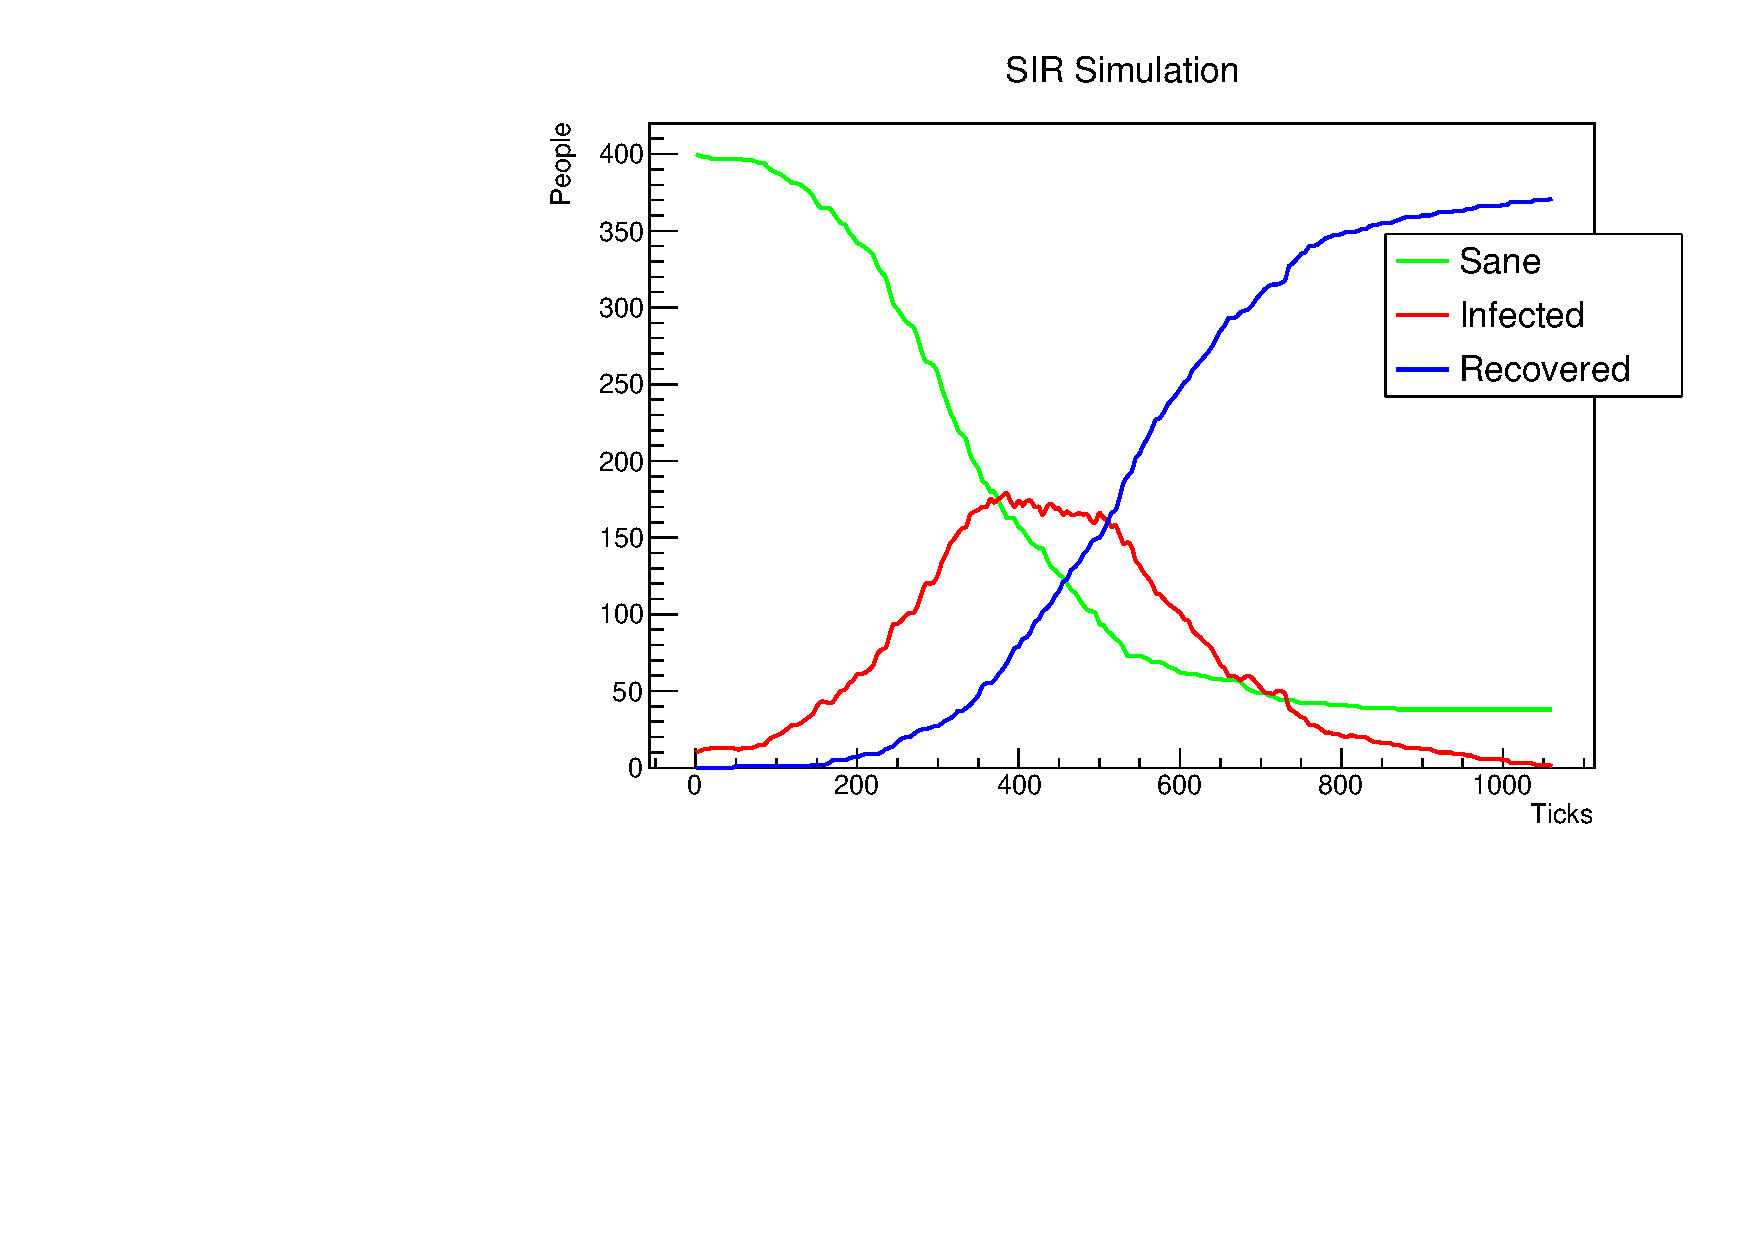
\includegraphics[width=0.5\textwidth]{images/simple_005.pdf}
    }
    \subfloat[][Probabilità: 0.08\label{fig:simple_008}]{
        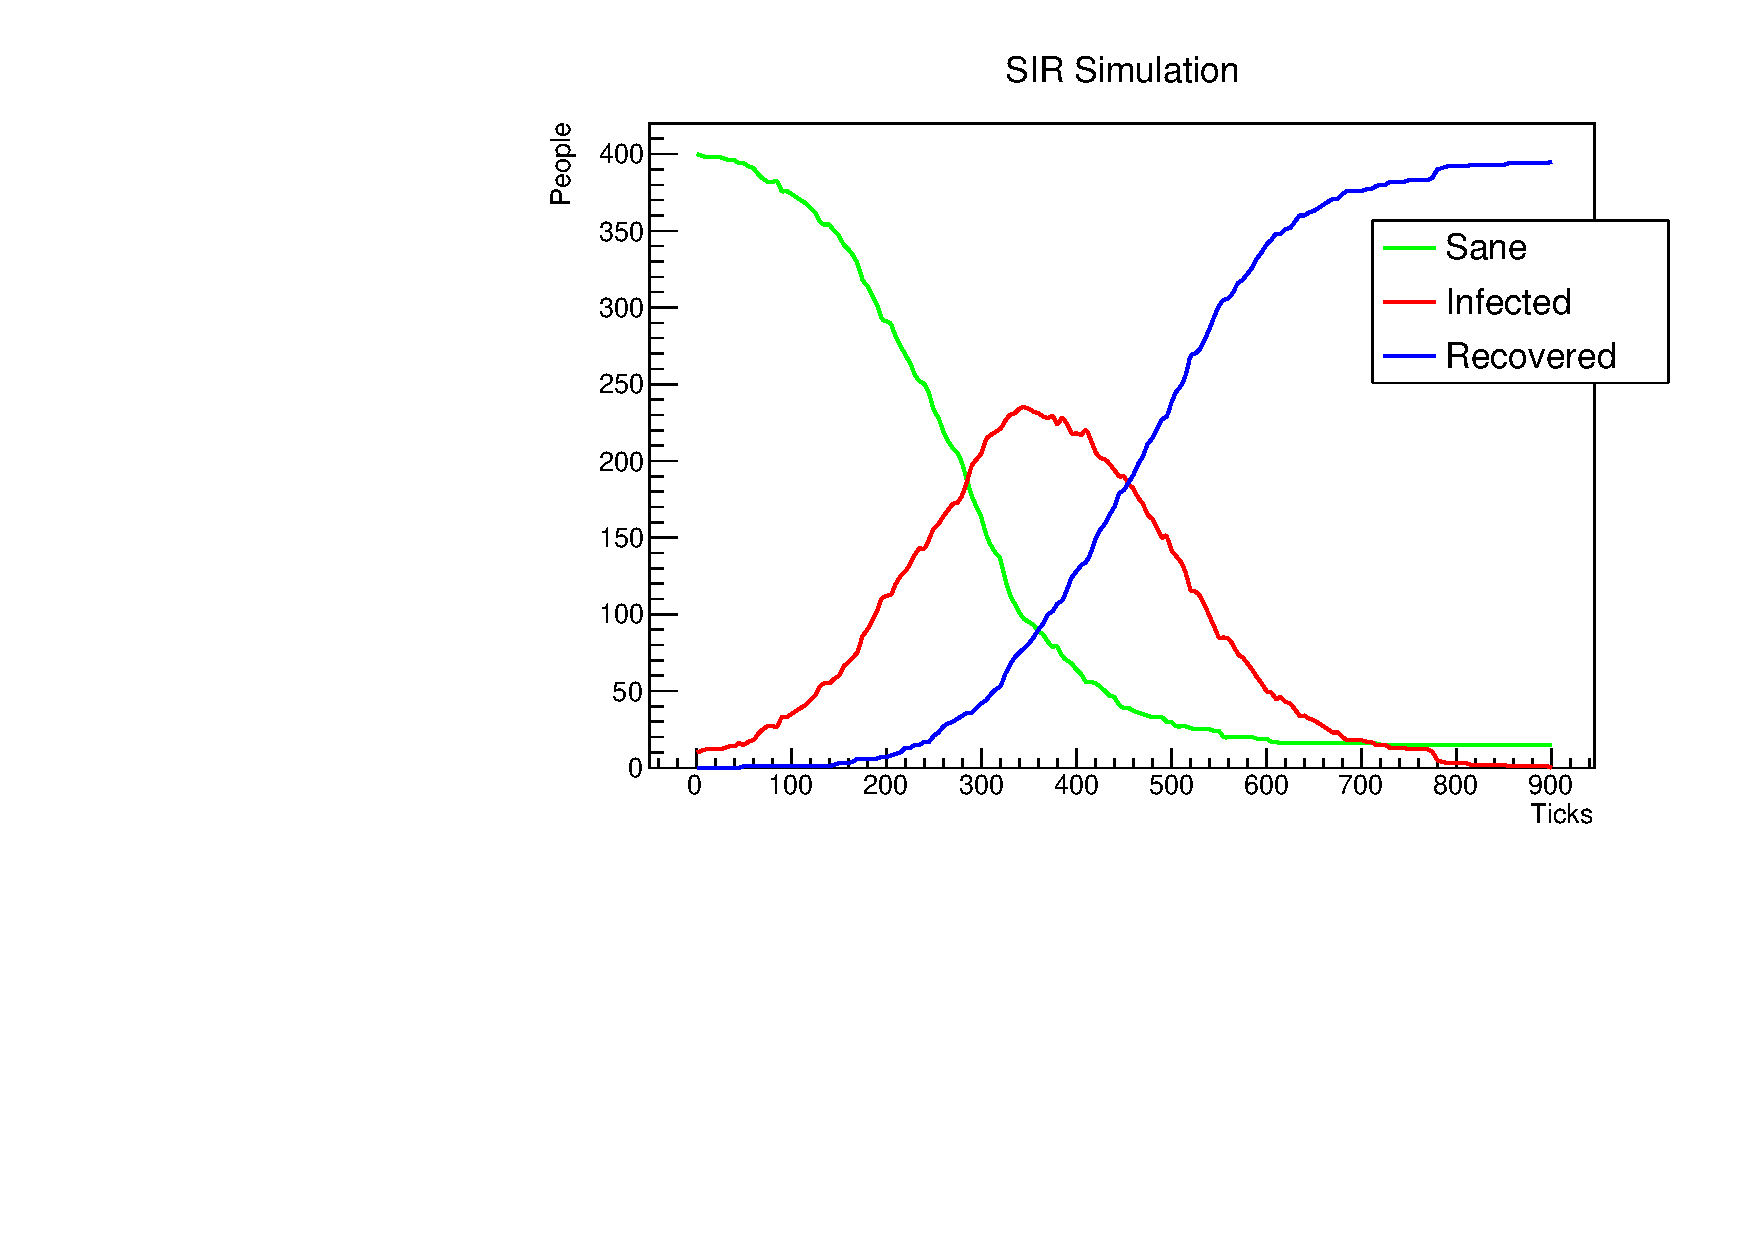
\includegraphics[width=0.5\textwidth]{images/simple_008.pdf}
    }
    \caption{Grafici di una simulazione con \emph{Simple Infection} a gestire l'infezione. I parametri della classe differiscono solo per la probabilità di infettarsi venendo a contatto con un individuo infettivo}
\end{figure*}

\begin{figure*}[p]
    \subfloat[][Size: 400\label{fig:simple_400}]{
        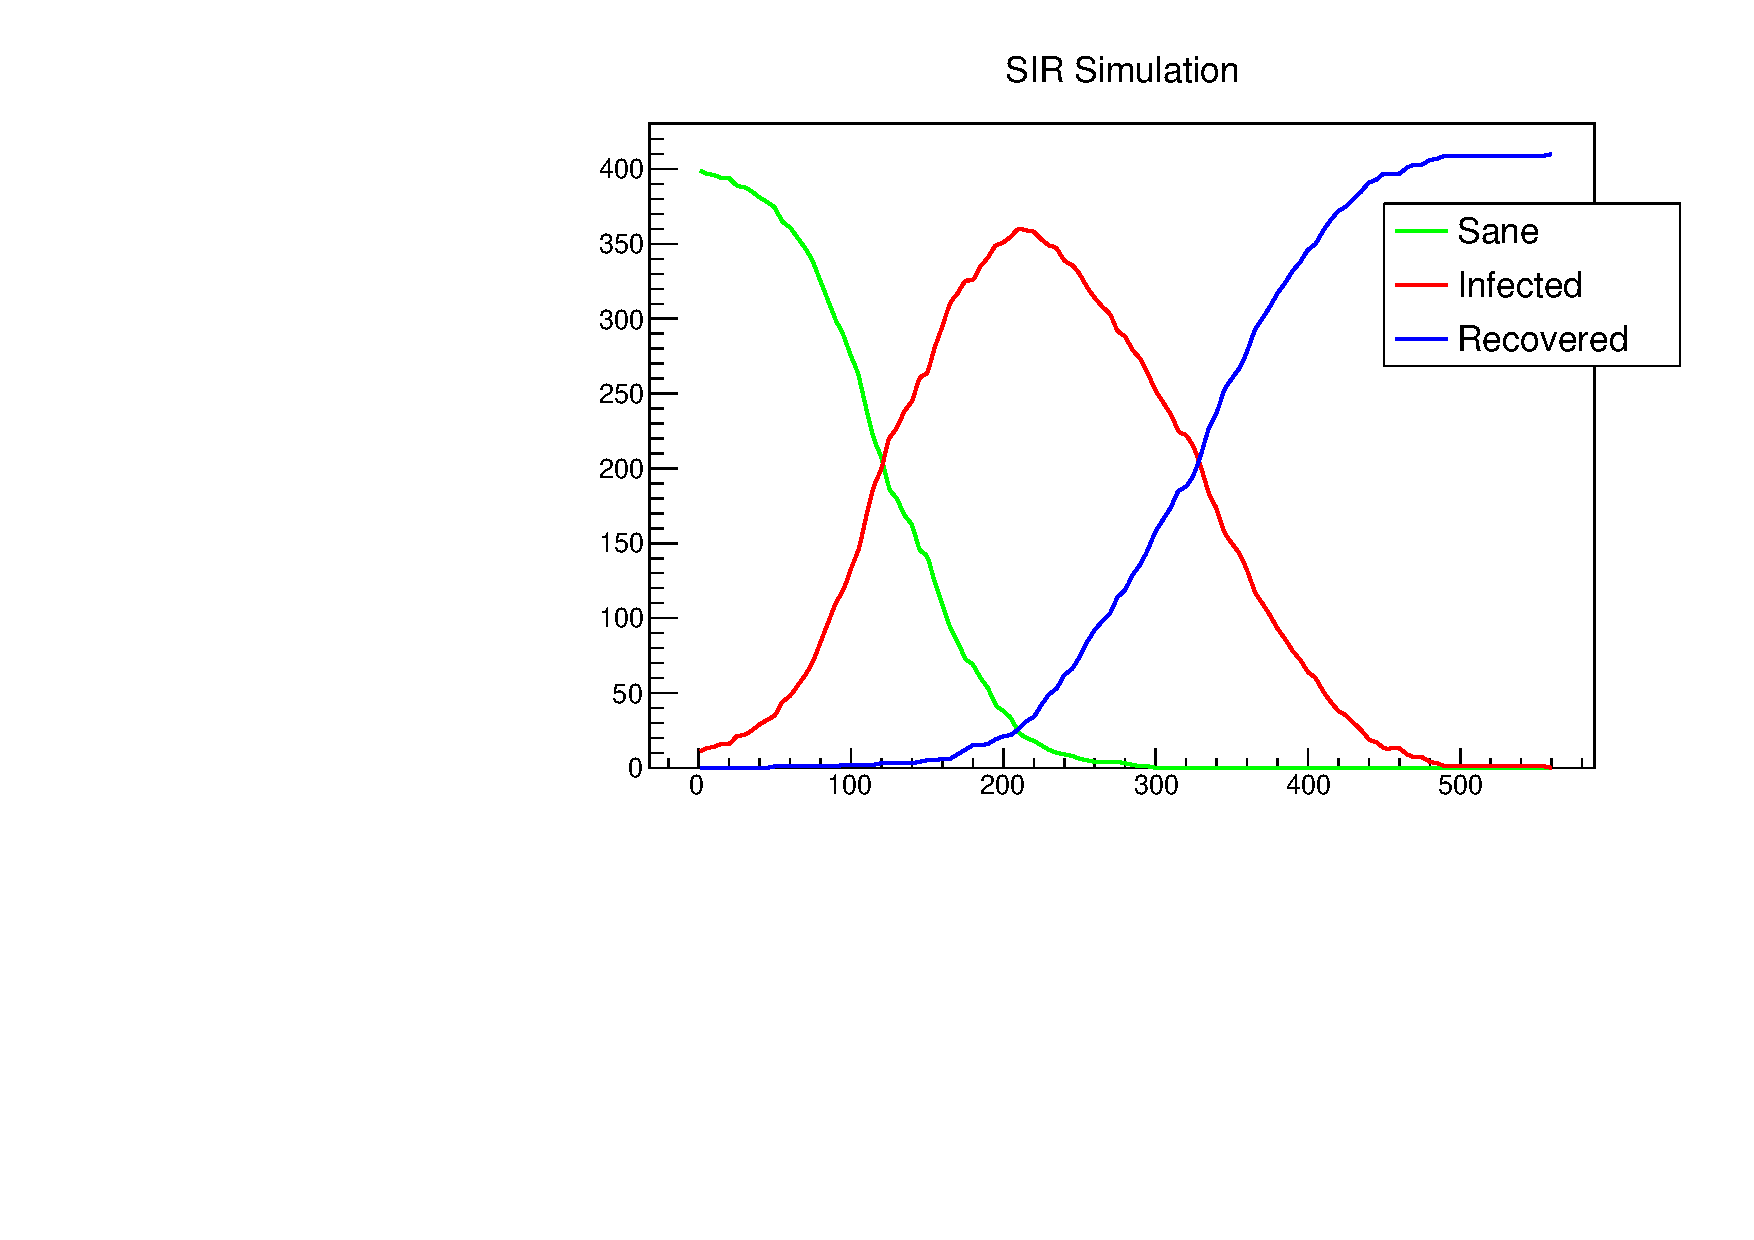
\includegraphics[width=0.5\textwidth]{images/simple_400.pdf}
    }
    \subfloat[][Size: 800\label{fig:simple_800}]{
        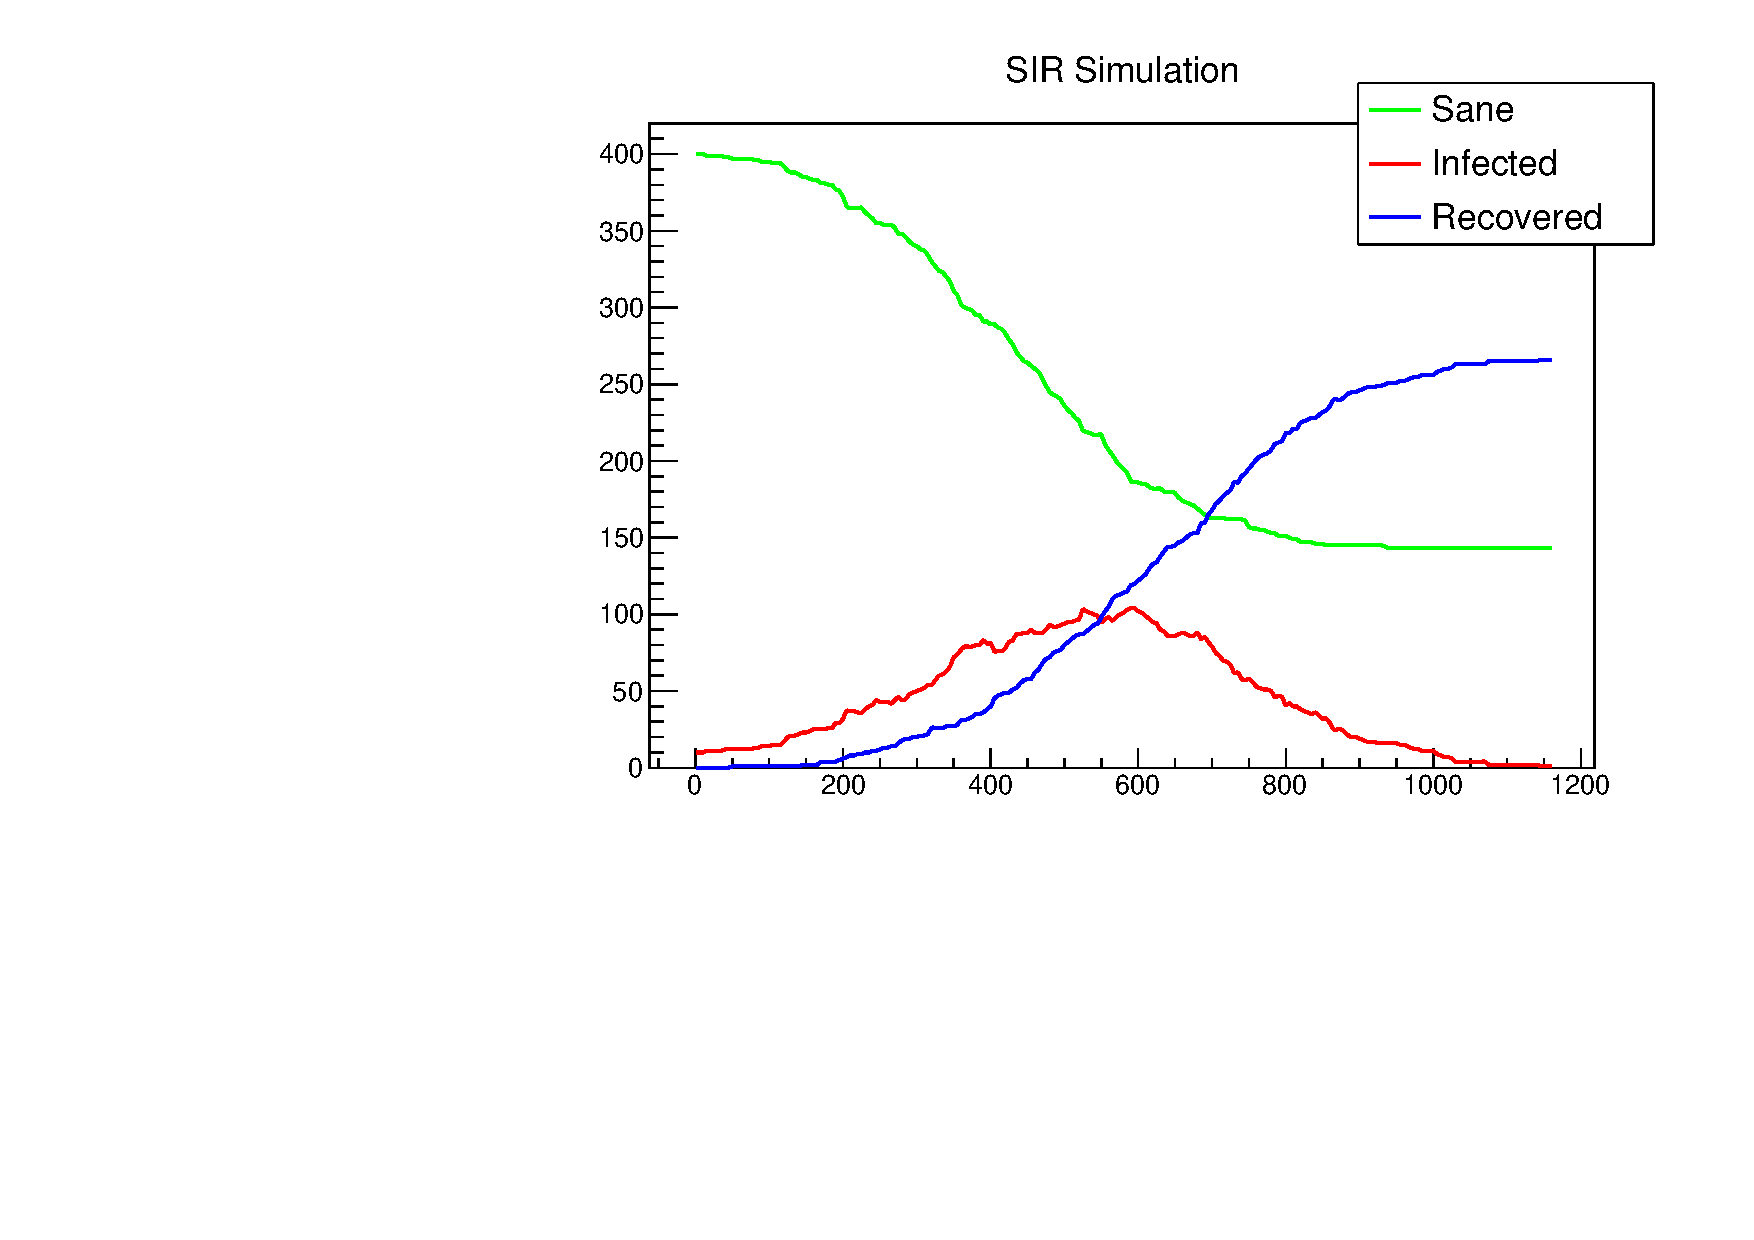
\includegraphics[width=0.5\textwidth]{images/simple_800.pdf}
    }
    \caption{Grafici di una simulazione con \emph{Simple Infection} a gestire l'infezione. I parametri della classe differiscono solo per la dimensione dello spazio a disposizione}
\end{figure*}

\begin{figure*}[p]
    \centering
    \subfloat[][Senza quarantena\label{fig:incubation}]{
        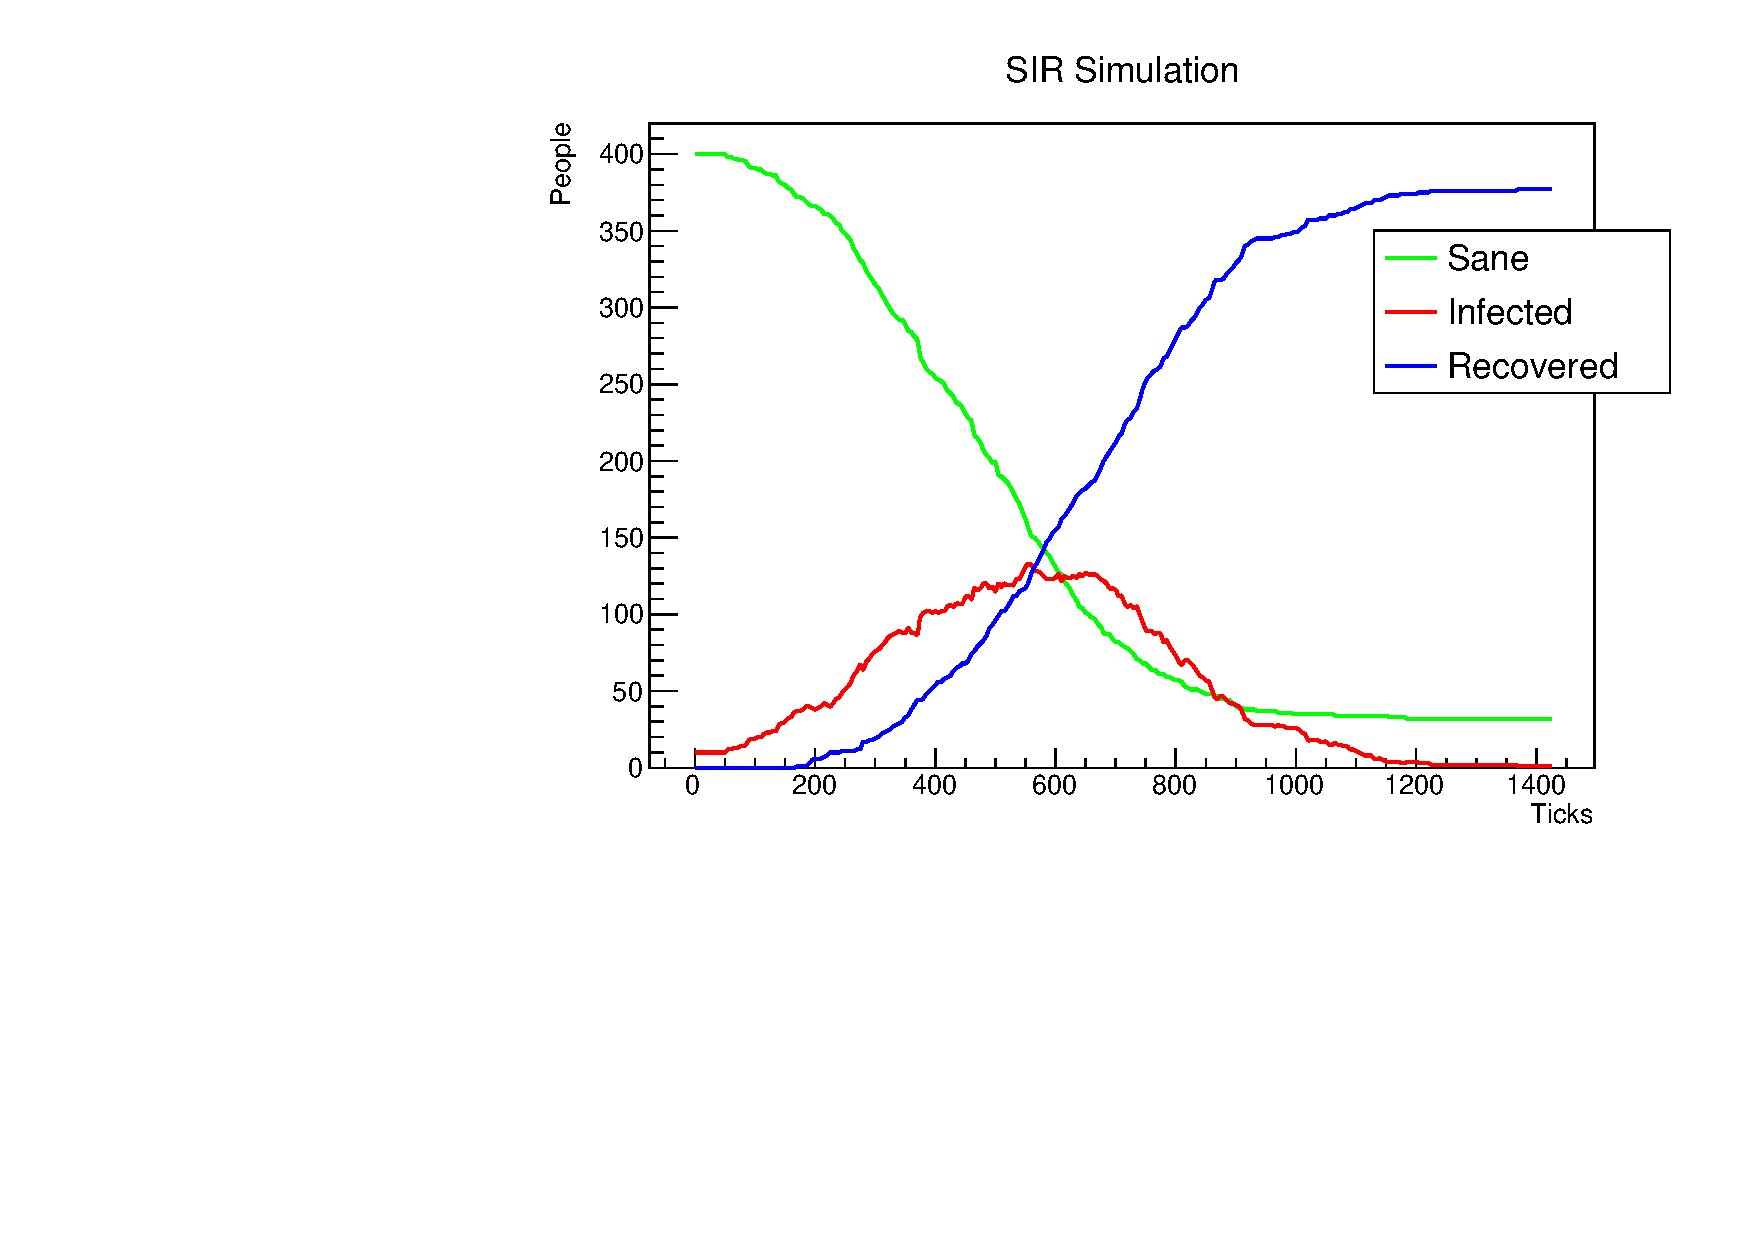
\includegraphics[width=0.5\textwidth]{images/incubation.pdf}
    }
    \subfloat[][Con quarantena\label{fig:quarantine}]{
        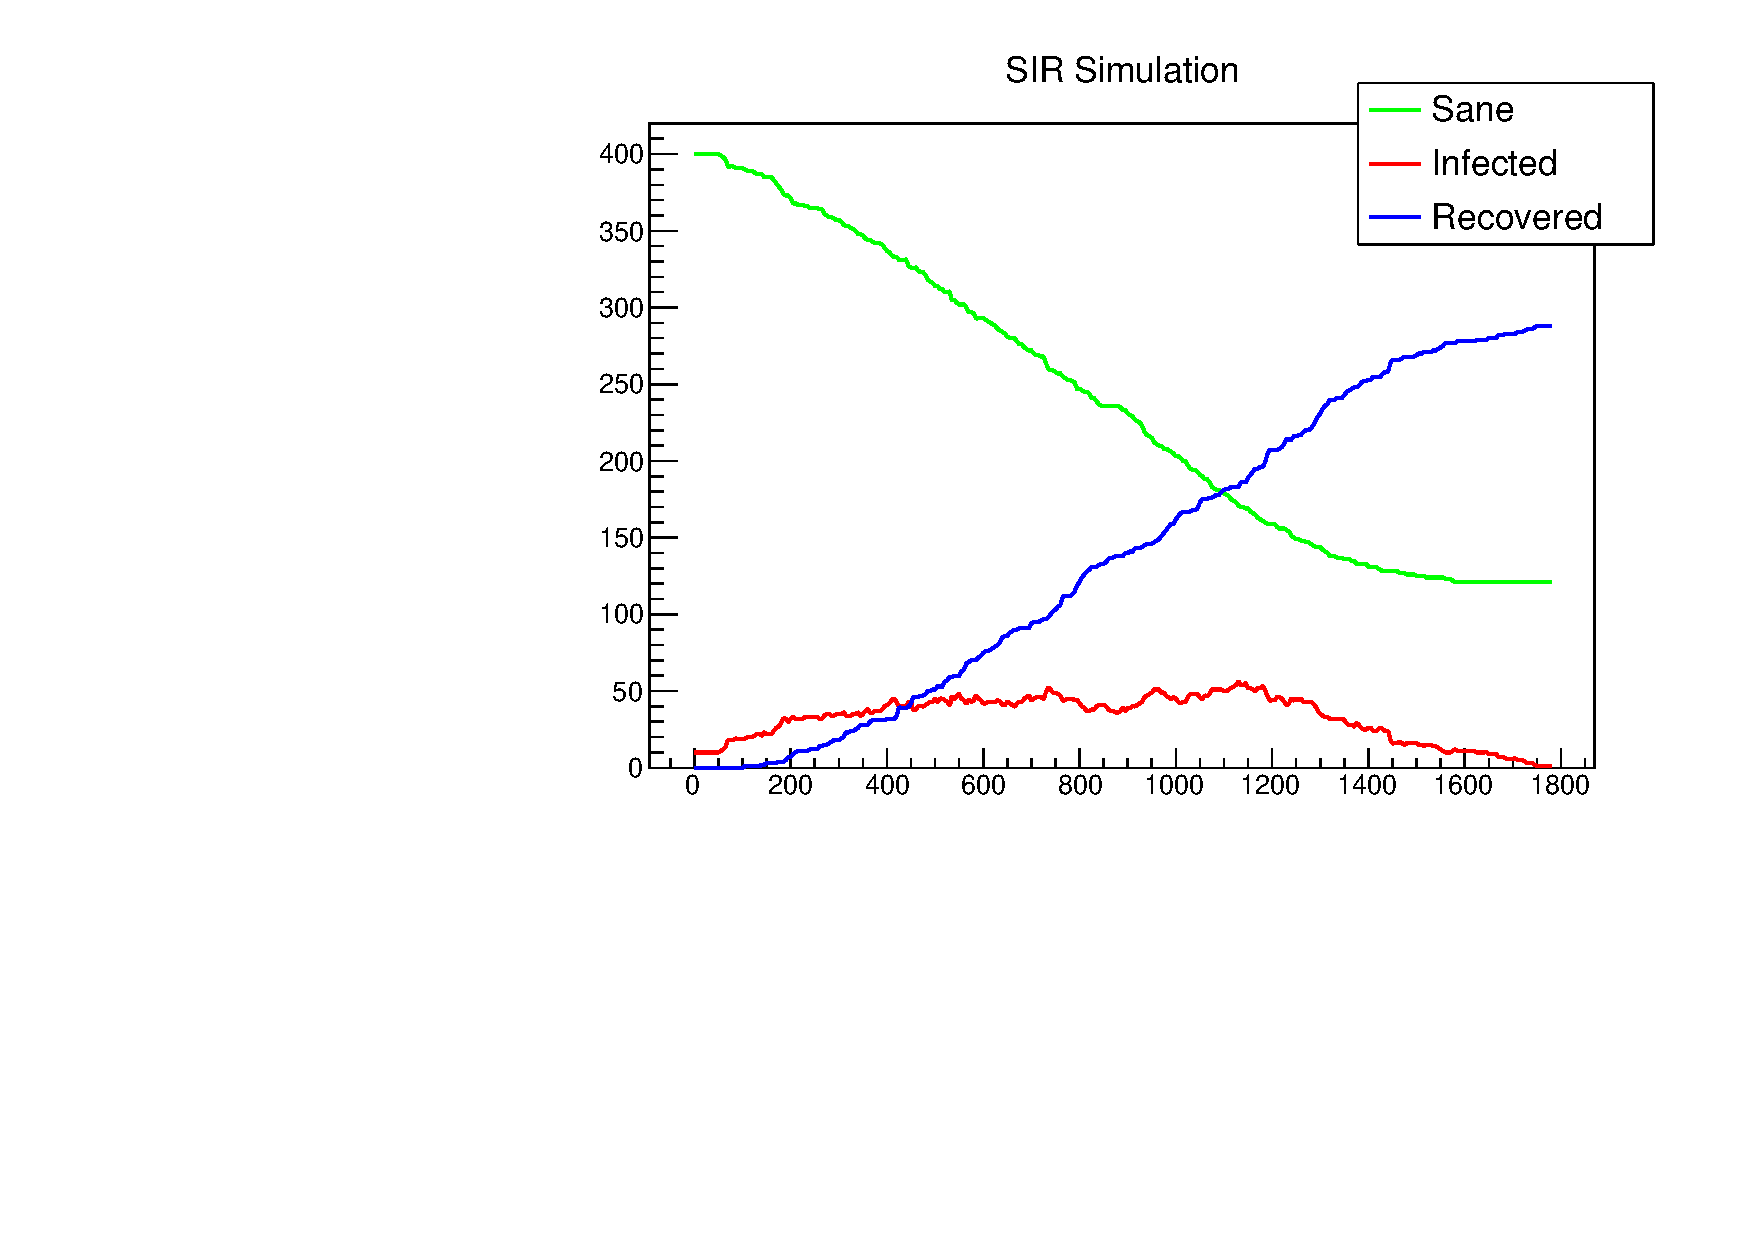
\includegraphics[width=0.5\textwidth]{images/quarantine.pdf}
    }
    \caption{Grafici di una simulazione con \emph{Incubation Infection} a gestire l'infezione. I parametri della classe sono gli stessi, ma nel secondo si è aggiunta la possibilità di essere costretti alla quarantena}
\end{figure*}

\section{Strategia di testing}
Per testare la correttezza del programma si è utilizzato Doctest. Si è scelto di testare esplicitamente solo le classi \emph{Motion} e \emph{Infection}, dato che costituiscono il cuore del programma e sono le più suscettibili ad errori. Per le classi \emph{Display} e \emph{Plot}, che gestiscono l'output grafico, ci si è limitati a verificarne il corretto funzionamento durante l'esecuzione del programma.

\subsection*{Motion}
Per testare la classe \emph{Motion}, si è creata un'istanza con deviazione standard nulla, così da poter prevedere lo spostamento delle persone. Si è poi generata una popolazione di un solo individuo e si è verificato che la posizione venisse aggiornata correttamente, tenendo conto della velocità iniziale, della presenza dell'attrito e degli urti con le pareti. In seguito si è creata una seconda istanza di \emph{Motion} con deviazione standard non nulla e si è controllato che le medie delle posizioni, velocità e accelerazioni della popolazione fossero compatibili con una distribuzione delle accelerazioni di media zero.

\subsection*{Infection}
Le due classi che gestiscono l'infezione sono state testate con popolazioni ridotte, senza aggiornare la posizione degli individui. Gli individui sono stati distanziati in modo da poter prevedere i contatti e i parametri probabilistici delle classi sono stati impostati in modo da generare eventi certi o impossibili. Si è poi verificato che i contagi avvenissero come previsto, controllando sia la composizione dei vettori sia il \emph{Sub Status} degli individui.

\begin{thebibliography}{9}
    \bibitem{bib:GitHub} Repository GitHub \url{https://github.com/lorenzomanini/SIR\_simulation}
    \bibitem{bib:CMake} CMake \url{https://cmake.org/}
    \bibitem{bib:SFML} SFML: Simple and Fast Multimedia Library \url{https://www.sfml-dev.org/}
    \bibitem{bib:ROOT} ROOT \url{https://root.cern.ch/}
\end{thebibliography}

\end{document}